\documentclass[a0]{sciposter}
%\usepackage[latin1]{inputenc}
\usepackage[T1]{fontenc}
\usepackage[utf8]{inputenc}
\usepackage{textcomp}
%\usepackage{hyperref}
\usepackage{lipsum}
\usepackage{epsfig}
\usepackage{amsmath}
\usepackage{amssymb}
\usepackage{multicol} 
\usepackage{graphicx,url}
\usepackage[english]{babel}   
\usepackage[svgnames]{xcolor}
\usepackage{empheq}
\usepackage[most]{tcolorbox}
\usepackage{anyfontsize}
\usepackage{t1enc}
%\usepackage[utf8]{inputenc} 
%\usepackage{fancybullets} 



\newtcbox{\mymath}[1][]{%
    nobeforeafter, math upper, tcbox raise base,
    enhanced, colframe=blue!30!black,
    colback=blue!30, boxrule=3pt,
    #1}


 \definecolor{qq}{rgb}{.6, 0.0, 0.99}
 
\renewcommand{\familydefault}{\rmdefault}
%\renewcommand{\titlefont}{\rmfamily}


%\setlength{\topmargin}{-4.5pc}
%\setlength{\rightmargin}{-8.5pc}
%\setlength{\leftmargin}{200.5pc}
%\setlength{\textheight}{1900mm}
%\setlength{\oddsidemargin }{-4.0pc}
\setlength{\textwidth}{790mm}
\setlength{\textheight}{1450mm} 

\setlength{\headheight}{0pt}
\setlength{\headsep}{-10.0pt}
\setlength{\topmargin}{-80.0pt}
\setlength{\oddsidemargin}{-80.0pt}


%\rightlogo[1]{ujlogo}
%\title{Lieb-Liniger model: emergence of dark solitons in the course of measurements of particle positions}
%Título do projeto

%\author{Andrzej Syrwid and Krzysztof Sacha}
%nome dos autores
%
\institute 
{Jagiellonian University in Kraków}
%Nome e endereço da Instituição

%\email{asyrwid@gmail.com}
% Onde você coloca os emails dos integrantes


%\date is unused by the current \maketitle


% Exibe os logos (direita e esquerda) 
% Procure usar arquivos png ou jpg, e de preferencia mantenha na mesma pasta do .tex
%%%%%%%%%%%%%%%%%%%%%%%%%%%%%%%%%%%%%%%%%%%%%%%%%%%%%%%%%%%%%%%%%%%%%%%%%%%%%%%%
%%% Begin of Document



\begin{document}
%define conference poster is presented at (appears as footer)

%\LEFTSIDEfootlogo  
% Uncomment to put footer logo on left side, and 
% conference name on right side of footer

% Some examples of caption control (remove % to check result)

%\renewcommand{\algorithmname}{Algoritme} % for Dutch

%\renewcommand{\mastercapstartstyle}[1]{\textit{\textbf{#1}}}
%\renewcommand{\algcapstartstyle}[1]{\textsc{\textbf{#1}}}
%\renewcommand{\algcapbodystyle}{\bfseries}
%\renewcommand{\thealgorithm}{\Roman{algorithm}}


\vspace{-0.5cm}
\center
\includegraphics[width=6.0cm]{ujlogo.pdf}	

\vspace{0.5cm}

%\begin{minipage}[l]{0.9\textwidth}
%\begin{flushleft}
\color{DarkBlue}
\center
\textbf{\Huge{Bayes' theorem and fluctuation theorems}
}

\color{black}
\vspace{0.9cm}

\textbf{\Large{Author:}} \Large{\underline{Micha\l{} Mandrysz}, \ Jagiellonian University in Krak\'{o}w}
\vspace{0.6cm}

% University/organization
%\end{flushleft}
%\end{minipage}
%\begin{minipage}[r]{0.1\textwidth}
%\includegraphics[width=6.0cm]{ujlogo.pdf}
%\end{minipage} 

%\begin{minipage}[b]{0.1\linewidth}
%\includegraphics[width=2.5cm]{ujlogo.pdf} % Logo or a photo of you, adjust its dimensions here
%\end{minipage}
%\begin{minipage}[b]{0.127\linewidth}
%\includegraphics[width=3.5cm]{ubial.jpg} % Logo or a photo of you, adjust its dimensions here
%\end{minipage}
%\begin{minipage}[b]{0.11\linewidth}
%\includegraphics[width=2.2cm]{ifpan.png} % Logo or a photo of you, adjust its dimensions here
%\end{minipage}



\vspace{1.0cm}

%%% Begin of Multicols-Enviroment


%%% Abstract
%\begin{abstract}
%\medium
Using Bayes' theorem we present a simple and general model which allows us to generate distributions of change in entropy between two macroscopic states. Obtained results are with agreement with the Second Law of thermodynamics, favouring decrease in the number of macroscopic states (keeping the number of microscopic states constant) and thus increasing the number of microscopic realisations of the surviving macrostates.
Due to the close resemblance of our expression to the fluctuation theorems we discuss its relation to Crooks Fluctuation Theorem. Surprisingly, the distributions obtained during experimental verification of Crooks relation on RNA strands follow closely the distributions obtained from our Bayesian relation.
%\end{abstract}

\begin{multicols}{3}


%====================================================================================================================================
%====================================================================================================================================
%====================================================================================================================================
%====================================================================================================================================

%%% Introduction
\section{Bayesian model for a generic physical system}
\normalsize
\begin{flushleft}
Consider a generic statistical mechanical system with a \textit{fixed} number of microstates, evolving under deterministic, microscopic equations of motion. 
\begin{itemize}
	\item $t_0$, $t_1$ - initial and final times
	\item $\{A_i\}, \{B_j\}$ - sets of initial and final macrostates
	\item $N_A, N_B$ - numbers of initial and final macrostates
	\item $M_i, N_j$ - numbers of microscopic realizations of $i$ initial and $j$ final macrostates.
	\item $K_{ij}$ - number of initial microstates of macrostate $A_i$ flowing into the final macrostate $B_j$, as illustrated on figure \ref{Fig4}.
\end{itemize}

\end{flushleft}

\begin{minipage}[b]{20.0cm}
\centering
\begin{figure}[ht!]
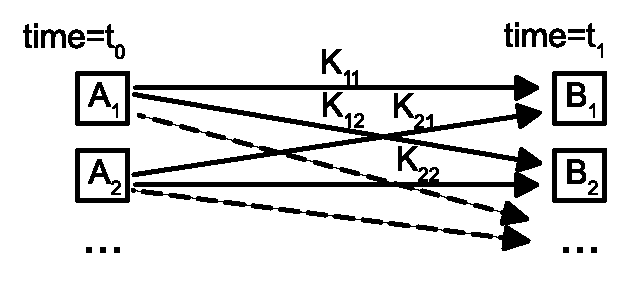
\includegraphics[width=20.0cm]{figure1.eps}
\caption{Transitions between macrostates ${A_i}$ and macrostate ${B_i}$ dictated by the 'transition' matrix $K_{ij}$.}
\label{Fig4} 
\end{figure}
\end{minipage}

\begin{flushleft}
The probability of the forward transition:
\begin{equation}
\label{ForwardProb}
  P(B_j|A_i)= \frac{K_{ij}}{M_i}.
\end{equation}
However, the probability of the time reversed case (post-diction) is given by the \textit{extended Bayes theorem}:
\begin{equation}
  P(A_i|B_j)=\frac{P(B_j|A_i)P(A_i)}{\sum_k P(B_j|A_k)P(A_k)}.
\end{equation}

Having no a priori knowledge about the initial macrostates, each of them is equally probable $P(A_i)= 1/N_A$, getting:

\begin{equation}
\begin{aligned}
  P(A_i|B_j) &= \frac{K_{ij}}{M_i} P(A_i) \left( \sum_k \frac{K_{kj}}{M_k}P(A_k) \right)^{-1}\\
  &= \frac{K_{ij}}{M_i} \left( \sum_{k} \frac{K_{kj}}{\sum_m K_{km}} \right)^{-1},
\end{aligned}
\end{equation}
\vspace{0.5cm}
\begin{tcolorbox}[colframe=green!500!white,colback=white!50!white,boxrule=3pt]
The conditional probabilities $P(B_j|A_i)$ and $P(A_i|B_j)$ are entirely different in nature - the first represents a prediction, but the second is a post-diction. There is no symmetry between assumptions and assertions in conditional probability calculus.
\end{tcolorbox}
\vspace{0.5cm}
The ratio of prediction and postdiction:

\begin{tcolorbox}[colframe=red!500!white,colback=white!50!white,boxrule=3pt]
\begin{equation}
\label{MacrostatesPRatio}
  \frac{P(B_j|A_i)}{P(A_i|B_j)}= e^{\ln{\sum_{k} \frac{K_{kj}}{\sum_m K_{km}}}}.
\end{equation}
\end{tcolorbox}
\vspace{0.5cm}

Natural interpretation of the term in the exponent is configurational (internal) entropy: 
\begin{tcolorbox}[colframe=green!500!white,colback=white!50!white,boxrule=3pt]
\begin{equation}
\Delta S_{conf} /k_B = \ln{\sum_{k} \frac{K_{kj}}{\sum_m K_{km}}} = - \beta \Delta F
\end{equation}
\end{tcolorbox}
\vspace{0.5cm}

In the limiting case of \textit{one} initial macrostate we recover the \textit{Boltzmann entropy}:

\begin{equation}
\Delta S_{conf} /k_B = \ln{\sum_{k} \frac{K_{kj}}{\sum_m K_{km}}} = \ln{\frac{N_j}{M_k}} =\Delta S_{B} /k_B
\end{equation}
\vspace{0.5cm}

With the increasing ratio of initial to final macrostates the probability of spontaneous return due to random heat fluctuations decreases indicating a generalization of the Second Law, quantifying the probability of reverse transitions. 
\vspace{0.5cm}

This feature is a general characteristics of the fluctuation theorems to which our result most likely belongs.
\end{flushleft}
\columnbreak
\begin{flushleft}
\section{General properties of obtained results}
Using random matrices filled with uniformly distributed integers from some interval $[0,Z], Z \in \mathbb{N}$, the following distributions were generated:

\begin{minipage}[b]{22.0cm}
\centering
\begin{figure}[ht!]
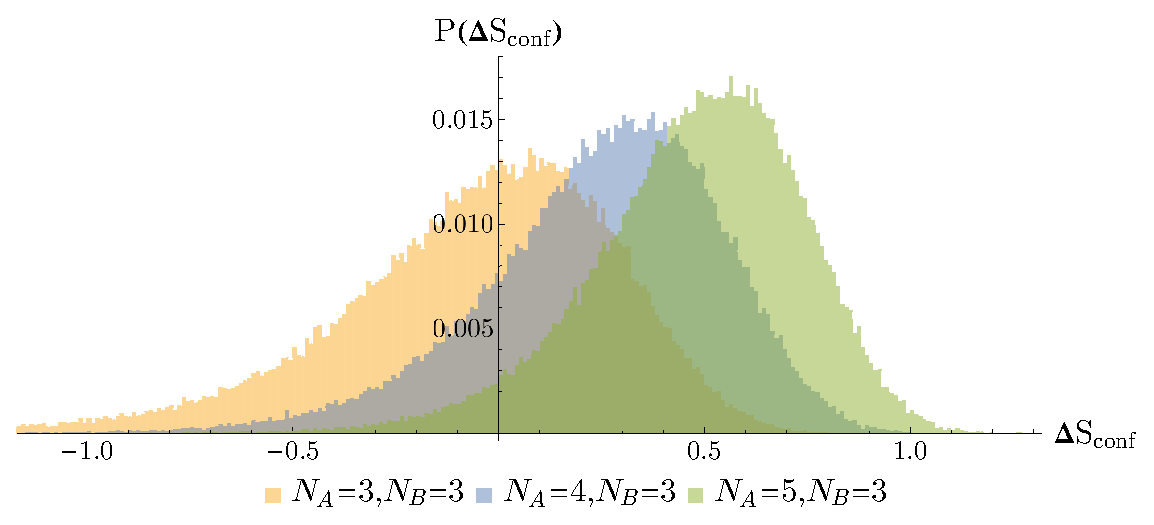
\includegraphics[width=22cm]{Figure2.eps} \caption{Probability distributions of change of entropy ($k_B =1$) in transitions between $N_A$ initial and $N_B$ final macrostates, calculations performed for $N=10^5$ random matrices.}
\label{Fig2} 
\end{figure}
\end{minipage}
\vspace{-0.5cm} 

Those results suggest that if our knowledge about the system stays in tact (no change in number of macroscopic states), then entropy most likely will not change (yellow graph from figure \ref{Fig2}). More importantly:

\vspace{0.6cm} 
\begin{tcolorbox}[colframe=green!500!white,colback=white!50!white,boxrule=3pt]
The preferred direction (higher entropy change) correlates with the fall in number of macroscopic (discernible) states and with growth of their microscopic realizations. In other words: The spontaneous direction of change is associated with an increasing number of inaccessible degrees of freedom.
\end{tcolorbox}


Comparison of the forward (spontaneous) to backward (non-spontaneous) distribution:

\begin{minipage}[b]{22.0cm}
\centering
\begin{figure}[ht!]
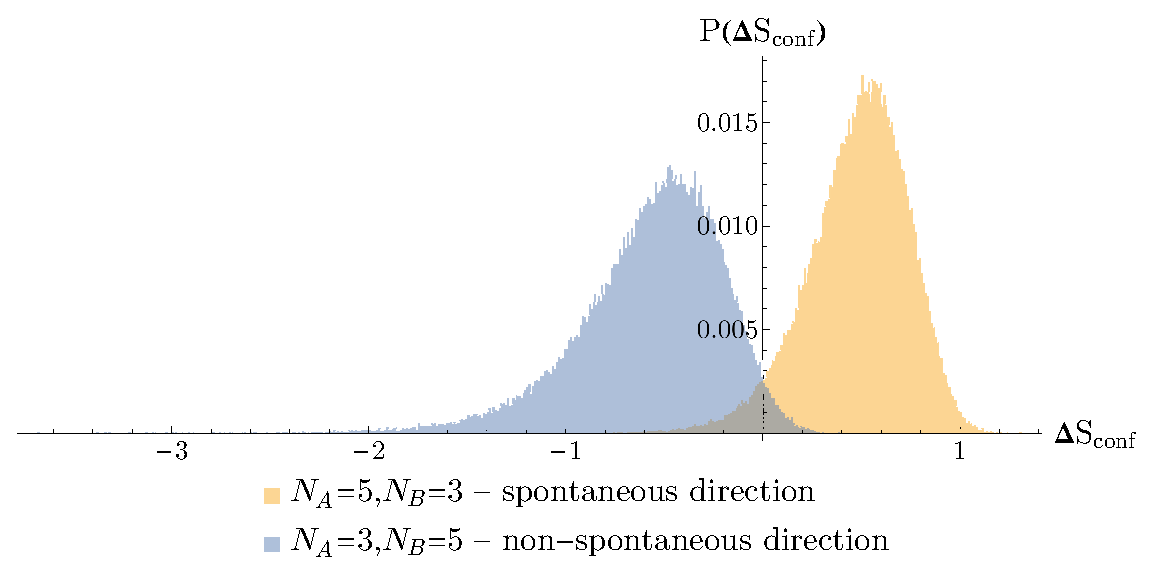
\includegraphics[width=22cm]{Figure3.eps} 
%\caption{Probability distributions of entropy produced ($k_B =1$) in transitions between $N_A$ initial and $N_B$ final macrostates, calculations performed for $N=10^5$ random matrices.}
\end{figure}
\end{minipage}
%\vspace{-1.0cm} 
\begin{minipage}[b]{22.0cm}
\centering
\begin{figure}[ht!]
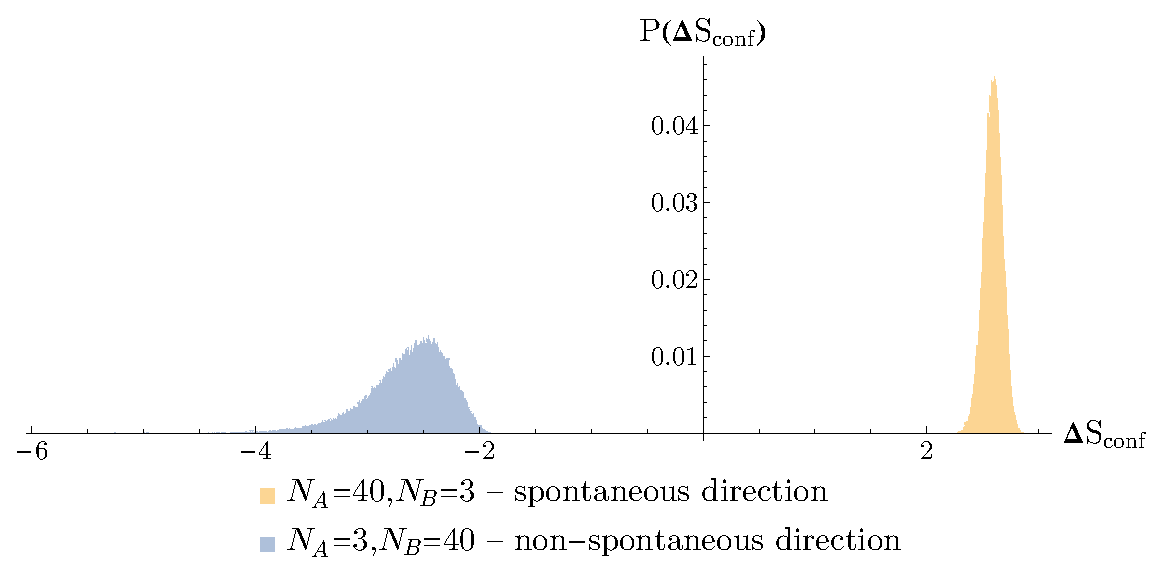
\includegraphics[width=22cm]{Figure4.eps} \caption{Probability distributions of change of entropy ($k_B =1$) in transitions between $N_A$ initial and $N_B$ final macrostates and the reverse scenarios.}
\label{Fig4} 
\end{figure}
\end{minipage}
\vspace{0.3cm} 

A general property observed from this results indicate: 

\vspace{0.3cm} 

\begin{tcolorbox}[colframe=green!500!white,colback=white!50!white,boxrule=3pt]
The nonspontaneous direction of change is associated with wider distributions of entropy change.
\end{tcolorbox}


\end{flushleft}

\columnbreak

\section{Our hypothesis}

\begin{minipage}[b]{22.0cm}
\centering
\begin{figure}[ht!]
 \includegraphics[clip, trim=10.5cm 19.5cm 1.0cm 2.1cm, width=20cm]{verification.pdf}
 \caption{Result obtained during experimental verification of Crooks Fluctuation theorem \cite{Collin:2005fxa}}
\label{Fig5} 

\end{figure}
\end{minipage}
\vspace{-1.0cm} 



%====================================================================================================================================
%====================================================================================================================================
%====================================================================================================================================
%====================================================================================================================================
\vspace{-0.5cm}

%\bibliographystyle{plain}
%\begin{thebibliography}{1}
\begin{small}
\vspace{-0.5cm}

\bibliographystyle{ieeetr}
\bibliography{Refs}
%\bibitem{syr1}A. Syrwid, K. Sacha, Phys. Rev. A \textbf{92}, 032110 (2015).
%
%\bibitem{syr2}A. Syrwid, M. Brewczyk, M. Gajda, K. Sacha, Phys. Rev. A \textbf{94}, 023623 (2016).
%
%\bibitem{syr3}A. Syrwid, K. Sacha, arXiv:1705.09607 (2017).

\end{small}

\end{multicols}

\end{document}